\documentclass[a4paper]{article}
\usepackage{pgf,tikz,pgfplots}
\usetikzlibrary{arrows,decorations.markings}
\pgfplotsset{compat=1.15}
\usepackage{mathrsfs}
\usetikzlibrary{arrows}
%% Language and font encodings
\usepackage[english]{babel}
\usepackage[utf8x]{inputenc}
\usepackage[T1]{fontenc}
\usepackage{float}
%% Sets page size and margins
\usepackage[a4paper,top=3cm,bottom=2cm,left=3cm,right=3cm,marginparwidth=1.75cm]{geometry}
\usepackage{fancyhdr}
\pagestyle{fancy}
%% Useful packages

\usepackage{amsmath}
\usepackage{amsthm}
\usepackage{enumitem}
\usepackage{eqnarray}
\usepackage{float}
\usepackage{esint}
\usepackage{wrapfig}
\usepackage{gensymb}
\usepackage{lipsum}
\usepackage{amssymb}
\usepackage{array}
\usepackage{tikz}
\usepackage[colorlinks=true, allcolors=blue]{hyperref}
\usepackage{graphicx}
\usepackage{amsmath}
\usepackage{amssymb}
\usepackage{graphicx}
\usepackage[colorlinks=true, allcolors=blue]{hyperref}
\usepackage{mathtools}
\DeclareMathOperator{\Proj}{Proj}
\DeclareMathOperator{\lcm}{lcm}
\DeclareMathOperator{\sinc}{sinc}
\DeclareMathOperator{\cosec}{cosec}
\DeclareMathOperator{\sgn}{sgn}
\DeclareMathOperator{\Span}{span}
\DeclareMathOperator{\nullity}{nullity}
\DeclarePairedDelimiter\floor{\lfloor}{\rfloor}
\DeclareMathOperator{\Res}{Res}
\DeclareMathOperator{\rank}{rank}
\DeclareMathOperator{\Ker}{Ker}
\DeclareMathOperator{\R}{R}
\DeclareMathOperator{\Tr}{Tr}
\DeclareMathOperator{\diag}{diag}
\DeclareMathOperator{\Log}{Log}
\DeclareMathOperator{\sech}{sech}
\DeclareMathOperator{\Var}{Var}
\newtheorem{ans}{Answer}

\definecolor{darkblue}{RGB}{	0, 0, 139}
\newtheoremstyle{new}% <name>
{2pt}% <Space above>
{2pt}% <Space below>
{\color{darkblue}}% Body font
{}% <Indent amount>
{\bfseries\color{black}}% Theorem head font
{:}% <Punctuation after theorem head>
{.5em}% <Space after theorem headi>
{}% <Theorem head spec (can be left empty, meaning `normal')>
\theoremstyle{new}
\newtheorem{qns}{Problem}
\setlength{\parindent}{0cm}
\title{\textbf{Part II EO Problem Sheet Solutions}}
\author{Tai Yingzhe, Tommy (ytt26)}
\date{}
\setlength{\parindent}{0cm}
\begin{document}
\maketitle
\tableofcontents
\newpage
\section{Problem Sheet 1}
\subsection*{Polarization}
\begin{qns}[Brewster angle]
Without using any special device, how can the direction of the polarizing axis of a polaroid sheet be determined?
\end{qns}
\begin{ans}
We need a natural source of polarized light, like the Sun, with a known polarization axis. The Brewster angle is defined as the angle of incidence where the reflection coefficient for light polarized parallel to the plane of incidence being zero. This is given by $\tan\theta_B=n_o/n$. For light travelling from air $(n_o=1)$ to a material of high refractive index $n$ (non-conducting and shiny surface), this will be close to 45\degree. As a result, light reflected at near 45\degree incidence from the surface is (mostly) vertically polarized. We then rotate the polaroid to a position where the transmission intensity is the minimum. The polarizing axis will be perpendicular to this orientation of the polaroid.
\end{ans}
\begin{qns}[Circular Polarization]
What are the time- and space-dependences of the electric and magnetic fields for light with the complex representations $E_+ = E_1 + iE_2$ and $E_-= E_1 − iE_2$, where $E_{1,2}$ represent the electric fields of $\pm z$-going waves of angular frequency $\omega$, linearly polarized along the $x$- and $y$-directions respectively.\\[5pt]
Classify $E_\pm$ as describing LCP or RCP light, distinguishing clearly between the cases of positive and negative wavevector $k_z$.
\end{qns}
\begin{ans}
We have
$$\mathbf{E_1}=E_0e^{i(kz-\omega t)}\mathbf{\hat{x}},\quad\mathbf{E_2}=E_0e^{i(kz-\omega t)}\mathbf{\hat{y}}$$
assuming $x$ and $y$ components have the same amplitude. We then have
$$\mathbf{E_+}=\mathbf{E_1}+i\mathbf{E_2}=E_0\begin{pmatrix}e^{i(kz-\omega t)}\\ie^{i(kz-\omega t)}\\0\\\end{pmatrix},\quad\mathbf{E_-}=\mathbf{E_1}-i\mathbf{E_2}=E_0\begin{pmatrix}e^{i(kz-\omega t)}\\-ie^{i(kz-\omega t)}\\0\\\end{pmatrix}$$
At $z=0$ and $t=0$ respectively, we deduce the temporal and spatial variation
$$\text{Re}[\mathbf{E_+}(z=0,t)]=E_0(\cos\omega t\mathbf{\hat{x}}+\sin\omega t\mathbf{\hat{y}}),\quad\text{Re}[\mathbf{E_+}(z,t=0)]=E_0(\cos kz\mathbf{\hat{x}}-\sin kz\mathbf{\hat{y}})$$
$$\text{Re}[\mathbf{E_-}(z=0,t)]=E_0(\cos\omega t\mathbf{\hat{x}}-\sin\omega t\mathbf{\hat{y}}),\quad\text{Re}[\mathbf{E_-}(z,t=0)]=E_0(\cos kz\mathbf{\hat{x}}+\sin kz\mathbf{\hat{y}})$$
The magnetic field will then be
$$\mathbf{H_+}=\frac{E_0}{Z_0}\begin{pmatrix}-ie^{i(kz-\omega t)}\\e^{i(kz-\omega t)}\\0\\\end{pmatrix},\quad\mathbf{H_-}=\frac{E_0}{Z_0}\begin{pmatrix}ie^{i(kz-\omega t)}\\e^{i(kz-\omega t)}\\0\\\end{pmatrix}$$
Again, at $z=0$ and $t=0$ respectively, we deduce the temporal and spatial variation
$$\text{Re}[\mathbf{H_+}(z=0,t)]=\frac{E_0}{Z_0}(-\sin\omega t\mathbf{\hat{x}}+\cos\omega t\mathbf{\hat{y}}),\quad\text{Re}[\mathbf{H_+}(z,t=0)]=\frac{E_0}{Z_0}(\sin kz\mathbf{\hat{x}}+\cos kz\mathbf{\hat{y}})$$
$$\text{Re}[\mathbf{H_-}(z=0,t)]=\frac{E_0}{Z_0}(\sin\omega t\mathbf{\hat{x}}+\cos\omega t\mathbf{\hat{y}}),\quad\text{Re}[\mathbf{H_-}(z,t=0)]=\frac{E_0}{Z_0}(-\sin kz\mathbf{\hat{x}}+\cos kz\mathbf{\hat{y}})$$
$\mathbf{E_+}$ is LCP for $k_z>0$ and RCP for $k_z<0$. $\mathbf{E_-}$ is RCP for $k_z>0$ and LCP for $k_z<0$.
\end{ans}
\newpage
\begin{qns}[Jones]
Show that the Jones matrix for a polaroid sheet with its transmitting axis at an angle $\theta$ to the $x$-axis is
$$J_\theta=\begin{pmatrix}\cos^2\theta&\sin\theta\cos\theta\\\sin\theta\cos\theta&\sin^2\theta\\\end{pmatrix}$$
\end{qns}
\begin{ans}
Since the polaroid sheet has the transmitting axis inclined $\theta$ to the $x$-axis, rays with polarization axis aligned with this transmission axis will pass through completely. The Jones vector representation of this transmitted ray is $j_1=(\cos\theta,\sin\theta)^T$. This ray is invariant under the action of the polaroid, with Jones matrix representation $J_\theta$, i.e. $J_\theta j_1=j_1$.\\[5pt]
On the other hand, rays with polarization axis aligned perpendicular to this transmission axis will not pass through. The Jones vector representation of the incident ray is $j_2=(\sin\theta,-\cos\theta)^T$. We must have $J_\theta j_2=0$.\\[5pt]
To find the Jones matrix $J_\theta$, we need to solve both
$$J_\theta\begin{pmatrix}\cos\theta\\\sin\theta\\\end{pmatrix}=\begin{pmatrix}\cos\theta\\\sin\theta\\\end{pmatrix},\quad J_\theta\begin{pmatrix}\sin\theta\\-\cos\theta\\\end{pmatrix}=\begin{pmatrix}0\\0\\\end{pmatrix}$$
which gives out desired result, unique up to a multiplicative factor. Here, $j_1$ and $j_2$ are eigenvectors of $J_\theta$ with eigenvalues 1 and 0 respectively.
\end{ans}
\begin{qns}[Birefringence]
Explain how a uniaxial birefringent material can be used to make a quarter-wave plate. If the principal refractive indices are $n_o$, $n_o$ and $n_e$, what is the minimum thickness the plate can be for light of free-space wavelength $\lambda$?
\end{qns}
\begin{ans}
The uniaxial birefringent material should be oriented with its principal axes such that $n_o$ and $n_e$ directions lie on the plane of incidence of the wave. To be a quarter-wave plate, the difference in phase it imparts on the fast and slow ray is exactly $\pi/2$. Consider an incident ray along the $z$-axis of the quarter-wave plate, then the introduced phase difference between the $x$-polarized and $y$-polarized component needs to be $\pi/2$ (or $(2n+1)\pi/2$ for $n\in\mathbb{Z}^+$), i.e.
$$J=\begin{pmatrix}e^{i\omega n_od/c}&0\\0&e^{i\omega n_ed/c}\\\end{pmatrix},\quad\Delta\phi=\frac{\omega}{c}|n_o-n_e|d=\frac{\pi}{2}\implies d=\frac{\lambda}{4|n_o-n_e|}$$
\end{ans}
\begin{qns}[Quarter wave plate]
A light beam is elliptically polarized with an axial ratio of 3 to 1 and the major axis vertical. What are the possible orientations of linearly polarized light which can be obtained by passing the beam through a quarter-wave plate?
\end{qns}
\begin{ans}
The Jones vector representation for an elliptically polarized ray is $(a,be^{i\delta})$. We are given $a=3$, $b=1$ and $\alpha=\pi/2$ (major axis vertical), where
$$\tan2\alpha=\frac{2ab}{a^2-b^2}\cos\delta\implies\cos\delta=0\implies\delta=\frac{\pi}{2}(2n+1)$$
So we have $(3,i)$. The Jones matrix for a quarter-wave plate (unique up to an unimportant multiplicative factor) is
$$J_{\lambda/4}=\begin{pmatrix}1&0\\0&\pm i\\\end{pmatrix}$$
where $\pm$ depends on the orientation of the fast and slow axes. This gives two possible linear polarizations:
$$\begin{pmatrix}1&0\\0&i\\\end{pmatrix}\begin{pmatrix}3\\i\\\end{pmatrix}=\begin{pmatrix}3\\-1\\\end{pmatrix}=\begin{pmatrix}1&0\\0&-i\\\end{pmatrix}\begin{pmatrix}3\\-i\\\end{pmatrix}$$
$$\begin{pmatrix}1&0\\0&-i\\\end{pmatrix}\begin{pmatrix}3\\i\\\end{pmatrix}=\begin{pmatrix}3\\1\\\end{pmatrix}=\begin{pmatrix}1&0\\0&i\\\end{pmatrix}\begin{pmatrix}3\\-i\\\end{pmatrix}$$
We then have these two possible orientations of linearly polarized light, with the vertical axis to be above and below, at an angle $\theta=\tan^{-1}(1/3)$ relative to the $x$-axis.
\end{ans}
\begin{qns}[Quarter wave plate, partially polarized]
When a light beam is passed through a linear polarizing filter, maximum and minimum intensities (5 and 2 units respectively) are found for vertical and horizontal planes of polarization. When the beam is passed through a quarter-wave plate with the fast axis vertical and then through the polarizing filter the maximum intensity is found at an angle of 26.6\degree to the vertical. What intensity is transmitted in this case? What is the degree of polarization before and after passing through the quarter-wave plate?
\end{qns}
\begin{ans}
If the light beam is purely polarized, then the ratio of intensities should have been 4 to 1, rather than 5 to 2. The optical components do not attenuate intensities. Hence, the light beam is partially polarized. Let the unpolarized intensity be $I_u$. The polarized part is given to have a maximum along the $y$-axis, so the most generic Jones vector representation is $(a,ib)$, where $b>a$. Given that the maximum and minimum intensities satisfy
$$5=b^2+I_u,\quad 2=a^2+I_u$$
The unpolarized part is unaffected by the quarter-wave plate. But, the polarized part after passing through the quarter wave plate, becomes linearly polarized
$$\begin{pmatrix}1&0\\0&-i\\\end{pmatrix}\begin{pmatrix}a\\ib\\\end{pmatrix}=\begin{pmatrix}a\\b\\\end{pmatrix}$$
at a given angle 26.6\degree$=\tan^{-1}(a/b)$ from the vertical, i.e. $a/b$ is the ratio of the amplitudes of the polarized components of the fields. From Fresnel-Arago laws, the unpolarized and polarized rays cannot interfere. The maximum intensity after the quarter-wave plate is $a^2+b^2+I_u$. Solve
$$a=b\tan26.6\degree,\quad 3=b^2-a^2,\implies b=\sqrt{\frac{3}{1-\tan^2(26.6\degree)}},\quad  a=\sqrt{3\bigg(\frac{1}{1-\tan^2(26.6\degree)}-1\bigg)}$$
which gives
$$I_u=5-b^2=2-a^2=5-\frac{3}{1-\tan^2(26.6\degree)}\implies a^2+b^2+I_u=\frac{3}{1-\tan^2(26.6\degree)}+2=6.004$$
and $a^2+b^2=5.008$. The degree of polarization before and after are respectively
$$\frac{b^2}{I_u+b^2}=\frac{4.004}{5}=0.8,\quad\frac{a^2+b^2}{I_u+a^2+b^2}=\frac{5.008}{6.004}=0.83$$
\end{ans}
\begin{qns}[Quarter wave plate]
Young’s double slit arrangement is illuminated with plane polarized, monochromatic light. The slits are covered by quarter-wave plates oriented to produce circular polarizations of opposite handedness. The “fringe” system is observed through a plane polarizing filter. What is observed as this filter is rotated?
\end{qns}
\begin{ans}
The quarter-wave plates placed in front of the slits produce circularly polarized light of opposite handedness. Two opposite-handed circular polarized rays give a linearly polarized ray when superposed. The orientation of polarization depends on the phase difference between them (related to the path difference $kd\sin\theta$ between the two rays in this double slit arrangement), i.e.
$$\mathbf{E_L}=E_0\begin{pmatrix}1\\i\\\end{pmatrix}e^{i(kx-\omega t)},\quad\mathbf{E_R}=E_0\begin{pmatrix}1\\-i\\\end{pmatrix}e^{i(kx-\omega t)}e^{i\Delta }\implies\mathbf{E}=\mathbf{E_L}+\mathbf{E_R}=E_0e^{i(kx-\omega t)}\begin{pmatrix}\cos\Delta /2\\\sin \Delta/2\\\end{pmatrix}$$
where $\Delta=kd\sin\theta$ and $d$ is the distance between the two slits. When two circular polarized waves are in quadrature (phase difference of $\pi/2$), the horizontal components constructively interfere and the vertical components destructively interfere. This gives a 'Fraunhofer diffraction pattern' of uniform intensity but with the direction of the polarization axis varying across the screen, i.e. fringes of alternating vertical and horizontal polarization. As the polarizing filter is rotated, the light fringes on the screen are shifted accordingly, i.e. a shift of one fringe spacing for every rotation of $\pi/2$ for the polarizer.
\end{ans}
\newpage
\begin{qns}[Optical elements]\leavevmode
\begin{enumerate}[label=(\alph*)]
\item Using Jones matrices, show that ideal crossed linear polarizers extinguish light of any polarization.
\item A quarter-wave plate is inserted between crossed polarizers, with its fast axis at an angle $\theta$ to the transmission axis Ox of the first polarizer. What is the resulting Jones matrix?
\item If unpolarized light of intensity $I$ is incident on this system, how does the transmitted intensity depend on $\theta$? What is the maximum transmitted intensity, and at what values of $\theta$ does this occur?
\end{enumerate}
\end{qns}
\begin{ans}\leavevmode
\begin{enumerate}[label=(\alph*)]
\item To extinguish light, $J_{\text{result}}$ must be the zero matrix, i.e.
$$J_{\text{result}}=J_xJ_y=\begin{pmatrix}1&0\\0&0\\\end{pmatrix}\begin{pmatrix}0&0\\0&1\\\end{pmatrix}=\boldsymbol{0}$$
\item Multiply the Jones matrix representations of all the optical elements involved:
$$J_yR_\theta J_{\lambda/4}R_\theta^{-1}J_x=\begin{pmatrix}0&0\\(1-i)\sin\theta\cos\theta&0\\\end{pmatrix}$$
\item After the first linear polarizer, the intensity is halved, so $\mathbf{E}=(1/\sqrt{2},0)$. The final field is
$$\mathbf{E_f}=J_yR_\theta e^{i\pi/4}\begin{pmatrix}1&0\\0&i\\\end{pmatrix}R_\theta^{-1}\begin{pmatrix}1/\sqrt{2}\\0\\\end{pmatrix}=\begin{pmatrix}0\\\sin\theta\cos\theta(1-i)\\\end{pmatrix}\frac{1}{\sqrt{2}}e^{i\pi/4}$$
The intensity is maximum at $\theta=\pi/4$ by inspection. the final intensity is $(1/\sqrt{2})^2(0.5I)=0.25 I$.
\end{enumerate}
\end{ans}
\begin{qns}[Double refraction]
A non-magnetic uniaxial crystal has principal refractive indices $n_o$, $n_o$ and $n_e$ in a Cartesian co-ordinate system with the z-axis aligned with the optic axis. A planewave with wavevector $\mathbf{k} = k(\sin\theta, 0, \cos \theta)$ has fields
$$\mathbf{D}(\mathbf{r},t)=D(-\cos\theta,0,\sin\theta)e^{i(\mathbf{k}\cdot\mathbf{r}-\omega t)}$$
$$\mathbf{H}(\mathbf{r},t)=H(0,1,0)e^{i(\mathbf{k}\cdot\mathbf{r}-\omega t)}$$
\begin{enumerate}[label=(\alph*)]
\item Find the corresponding $\mathbf{E}$ and $\mathbf{B}$ fields, and show that these fields satisfy all of Maxwell’s Equations provided the speed of the wave is $c/n_b$, with
$$\frac{n_b^2\sin^2\theta}{n_e^2}+\frac{n_b^2\cos^2\theta}{n_p^2}=1$$
\item What is the direction of the Poynting vector?
\end{enumerate}
\end{qns}
\newpage
\begin{ans}\leavevmode
\begin{enumerate}[label=(\alph*)]
\item The dielectric tensor is $\varepsilon=\diag(n_o^2,n_o^2,n_e^2)$ since the optic axis is given to be along $z$. We have
$$\mathbf{E}=\frac{1}{\varepsilon_0}\varepsilon^{-1}\mathbf{D}=\frac{D}{\varepsilon_0}e^{i(\mathbf{k}\cdot\mathbf{r}-\omega t)}\begin{pmatrix}-\cos\theta/n_o^2\\0\\\sin\theta/n_e^2\\\end{pmatrix},\quad\mathbf{B}=\mu_0\mathbf{H}=\mu_0H\begin{pmatrix}0\\1\\0\\\end{pmatrix}e^{i(\mathbf{k}\cdot\mathbf{r}-\omega t)}$$
The Maxwell equations in matter (with no free charges and current) are
$$\boldsymbol{\nabla}\cdot\mathbf{D}=0,\quad\boldsymbol{\nabla}\cdot\mathbf{B}=0,\quad\boldsymbol{\nabla}\times\mathbf{E}=-\mathbf{\dot{B}},\quad\boldsymbol{\nabla}\times\mathbf{H}=\mathbf{\dot{D}}$$
For EM waves, we could simplify $\boldsymbol{\nabla}$ using $\mathbf{k}$ and $\omega$. We have
$$\boldsymbol{\nabla}\cdot\mathbf{D}=\mathbf{k}\cdot\mathbf{D}=kD\begin{pmatrix}\sin\theta\\0\\\cos\theta\\\end{pmatrix}\cdot\begin{pmatrix}-\cos\theta\\0\\\sin\theta\\\end{pmatrix}e^{i(\mathbf{k}\cdot\mathbf{r}-\omega t)}=kDe^{i(\mathbf{k}\cdot\mathbf{r}-\omega t)}(-\cos\theta\sin\theta+\sin\theta\cos\theta)=0$$
$$\boldsymbol{\nabla}\cdot\mathbf{B}=\mathbf{k}\cdot\mathbf{B}=\mu_0Hk\begin{pmatrix}\sin\theta\\0\\\cos\theta\\\end{pmatrix}\cdot\begin{pmatrix}0\\1\\0\\\end{pmatrix}e^{i(\mathbf{k}\cdot\mathbf{r}-\omega t)}=0$$
$$\boldsymbol{\nabla}\times\mathbf{E}=-\mathbf{\dot{B}}\implies\mathbf{k}\times\mathbf{E}=\omega\mathbf{B},\quad\boldsymbol{\nabla}\times\mathbf{H}=\mathbf{\dot{D}}\implies\mathbf{k}\times\mathbf{H}=-\omega\mathbf{D}$$
Check LHS for Faraday's equation:
$$\mathbf{k}\times\mathbf{E}=\begin{vmatrix}\mathbf{\hat{x}}&\mathbf{\hat{y}}&\mathbf{\hat{z}}\\\sin\theta&0&\cos\theta\\-\cos\theta/n_o^2&0&\sin\theta/n_e^2\\\end{vmatrix}\frac{Dk}{\varepsilon_0}e^{i(\mathbf{k}\cdot\mathbf{r}-\omega t)}=-\mathbf{\hat{y}}\bigg(\frac{\cos^2\theta}{n_o^2}+\frac{\sin^2\theta}{n_e^2}\bigg)\frac{Dk}{\varepsilon_0}e^{i(\mathbf{k}\cdot\mathbf{r}-\omega t)}$$
and RHS for Faraday's law: $\omega\mathbf{B}=\mu_0\omega H\mathbf{\hat{y}}e^{i(\mathbf{k}\cdot\mathbf{r}-\omega t)}$. Faraday's Law is satisfied if 
$$\frac{\cos^2\theta}{n_o^2}+\frac{\sin^2\theta}{n_e^2}=-\mu_0\varepsilon_0\frac{\omega}{k}\frac{H}{D}$$
Check LHS for Ampere's law:
$$\mathbf{k}\times\mathbf{H}=\begin{vmatrix}\mathbf{\hat{x}}&\mathbf{\hat{y}}&\mathbf{\hat{z}}\\\sin\theta&0&\cos\theta\\0&1&0\\\end{vmatrix}kHe^{i(\mathbf{k}\cdot\mathbf{r}-\omega t)}=\begin{pmatrix}-\cos\theta\\0\\\sin\theta\\\end{pmatrix}kHe^{i(\mathbf{k}\cdot\mathbf{r}-\omega t)}$$
and RHS for Ampere's Law: $\mathbf{D}=D(-\mathbf{\hat{x}}\cos\theta+\mathbf{\hat{z}}\sin\theta)e^{i(\mathbf{k}\cdot\mathbf{r}-\omega t)}$. For Ampere's Law to be satisfied, we must have $\frac{H}{D}=-\omega/k$. This is true since $\mathbf{k}\times\mathbf{H}=-\omega\mathbf{D}$ (exactly one of $\mathbf{k}$, $\mathbf{H}$ and $\mathbf{D}$ must be negative since $\{\mathbf{k},\mathbf{H},\mathbf{D}\}$ form a left-handed set) Hence,
$$\frac{\cos^2\theta}{n_o^2}+\frac{\sin^2\theta}{n_e^2}=-\frac{1}{c^2}\frac{\omega}{k}\bigg(-\frac{\omega}{k}\bigg)=\frac{1}{n_b^2}$$
where $\omega/k=c/n_b$ is the speed of the wavelet, with $n_b$ being an effective refractive index for the plane wave with arbitrary wavevector $\mathbf{k}$.
\item The Poynting vector is
$$\mathbf{N}=\frac{1}{2}\text{Re}[\mathbf{E}\times\mathbf{H}^*]=\frac{DH}{2\varepsilon_0}\begin{vmatrix}\mathbf{\hat{x}}&\mathbf{\hat{y}}&\mathbf{\hat{z}}\\-\cos\theta/n_o^2&0&\sin\theta/n_e^2\\0&1&0\\\end{vmatrix}=\frac{DH}{2\varepsilon_0}\begin{pmatrix}-\sin\theta/n_e^2\\0\\-\cos\theta/n_o^2\\\end{pmatrix}$$
In the limit of $n_o\approx n_e$, then $\mathbf{N}$ is anti-parallel to $\mathbf{k}$.
\end{enumerate}
\end{ans}
\begin{qns}[Optical activity]
Born has demonstrated that a “molecule” composed of four identical polarizable spheres, interacting by Coulomb fields, can produce optical rotation. Would this be true if the spheres were at the corners of a regular tetrahedron? Might one expect optical rotation from a tri-atomic molecule?
\end{qns}
\begin{ans}
Regular tetrahedral molecule may be chiral (its mirror image cannot be superimposed with the original) only if we have 4 different groups. In this case, it is not. A triatomic molecule can never be chiral.
\end{ans}
\newpage
\begin{qns}[Optical activity]
An EM cavity of length $L$ in the $z$-direction is formed between two perfect plane mirrors. What are the frequencies of the cavity modes (i.e. the standing waves of light with wavevector parallel to the $z$-axis) in the cases where the cavity contains:
\begin{enumerate}[label=(\alph*)]
\item a non-magnetic uniaxial crystal with principal refractive indices $n_o$ and $n_e$ with the optic axis aligned (i) parallel; (ii) perpendicular to the z-axis;
\item an optically active material with average refractive index $n$ and specific rotatory power $\alpha$;
\item a Faraday medium with average refractive index $n$ and Verdet constant $\mathcal{V}$ with a magnetic field $\mathbf{B}$ along the $z$-axis.
\end{enumerate}
\end{qns}
\begin{ans}\leavevmode
\begin{enumerate}[label=(\alph*)]
\item Consider an EM wave of electric field 
$$\mathbf{E}=\mathbf{\hat{x}}(E_1e^{ik_1z}+E_2e^{-ik_2z})e^{-i\omega t}+\mathbf{\hat{y}}(E_3e^{ik_3z}+E_4e^{-ik_4z})e^{-i\omega t}$$
The dielectric tensors for (i) and (ii) respectively are $\diag(n_o,n_o,n_e)$ and $\diag(n_e,n_o,n_o)$. Apply boundary conditions for $\mathbf{E}=\boldsymbol{0}$ at $z=0$ and $z=L$ respectively: 
$$E_1+E_2=0,\quad E_3+E_4=0$$
$$k_{1,2}=\frac{m\pi}{L},\quad k_{3,4}=\frac{m'\pi}{L},\quad m,m'\in\mathbb{Z}$$
For (i), it will just be $k_1=k_2=k_3=k_4=\frac{\omega n_o}{c}$, and hence a single frequency $\omega=\frac{m\pi c}{Ln_o}$. For (ii), it will be $k_1=k_2=\omega n_o/c$ and $k_3=k_4=\omega n_e/c$, according to the dielectric tensor. There is thus two frequencies:
$$\text{ along }\mathbf{\hat{y}}:~\omega_0=\frac{c\pi m}{Ln_o},\quad\text{ along }\mathbf{\hat{x}}:~\omega_e=\frac{c\pi m'}{L n_e}$$
\item By definition of chiral materials, 
$$n_L=n_0+\frac{c\alpha}{\omega},\quad n_R=n_0-\frac{c\alpha}{\omega}$$
The electric field of the EM wave is
$$\mathbf{E}=E_1\begin{pmatrix}1\\i\\0\\\end{pmatrix}e^{i(k_1z-\omega t)}+E_4\begin{pmatrix}1\\-i\\0\\\end{pmatrix}e^{-i(k_1z+\omega t)}+E_2\begin{pmatrix}1\\i\\0\\\end{pmatrix}e^{-i(k_2z+\omega t)}+E_3\begin{pmatrix}1\\-i\\0\\\end{pmatrix}e^{i(k_3z-\omega t)}$$
where the first two terms are LCP and the last two terms are RCP. We also have $k_1=k_4=\omega n_L/c$ and $k_2=k_3=\omega n_R/c$. Apply boundary conditions for $\mathbf{E}=\boldsymbol{0}$ at $z=0$ and $z=L$:
$$E_1+E_2+E_3+E_4=0,\quad E_1+E_2-E_3-E_4=0\implies E_1=-E_2,~E_3=-E_4$$
$$k_1+k_2=\frac{2\pi m}{L},\quad k_3+k_4=\frac{2\pi m}{L},\quad m\in\mathbb{Z}$$
We then have $\omega(n_R+n_L)=2\pi mc/L\implies\omega=\frac{2\pi cm}{(n_L+n_R)L}=\frac{\pi cm}{nL}$.
\item By definition, we have $\theta=\mathcal{V}Bd=\frac{\omega}{2c}(n_L-n_R)d$, we then have
$$n_L=n+\frac{\mathcal{V}Bc}{\omega},\quad n_R=n-\frac{\mathcal{V}Bc}{\omega}$$
We then have $k_1=\frac{\omega n_R}{c}=k_2$ and $k_3=\frac{\omega n_L}{c}=k_4$. Apply boundary conditions again, we finally have
$$\omega_{1,2}=\frac{m\pi c}{nL}+\frac{\mathcal{V}Bc}{n},\quad\omega_{3,4}=\frac{m\pi c}{nL}-\frac{\mathcal{V}Bc}{n},\quad m\in\mathbb{Z}$$
\end{enumerate}
\end{ans}
\begin{qns}[Optical activity]
Show that for a plasma in a magnetic field $\mathbf{B}$ at low frequencies ($\omega<<\omega_c$, $\omega<<\omega_p^2/\omega_c$), where $\omega_p$ and $\omega_c$ is the plasma and cyclotron frequencies) there exist propagating LCP modes with wavevector $\mathbf{k}\parallel\mathbf{B}$, but no such propagating RCP modes. Derive the dispersion relation of the propagating modes at low frequency, and obtain an expression for their group velocity.\\[5pt]
[The propagating modes are “helicon” modes, and are responsible for “whistlers”, a characteristic type of audio-frequency radio interference most commonly encountered at high latitudes. They are brief, intermittent pulses at audible frequencies, rapidly descending in pitch.]
\end{qns}
\newpage
\begin{ans}
This is a plasma with field $\mathbf{B}=B_0\mathbf{\hat{z}}$ in Faraday geometry $\mathbf{k}\parallel\mathbf{B}$. The electron's equation of motion is
$$m\mathbf{\ddot{r}}=-e(\mathbf{E}+\mathbf{\ddot{r}}\times\mathbf{B})$$
Try LCP: $\mathbf{E}=E(1,i)^Te^{-i\omega t}\implies\mathbf{r}=a(1,i)^Te^{-i\omega t}$, then we have
$$\omega^2a=\frac{eE}{m}+a\omega\omega_c$$
The polarization in plasma is $\mathbf{P}=-ena(1,i)^T=\varepsilon_0\chi_LE(1,i)^T$ where $n$ is the number of electrons per unit volume. We then have
$$\chi_L=-\frac{ena}{\varepsilon_0E}=-\frac{e^2na}{\varepsilon_0ma(\omega^2-\omega\omega_c)}=-\frac{\omega_p^2}{\omega^2-\omega\omega_c}\sim\frac{\omega_p^2}{\omega\omega_c}>>1$$
We then have the refractive index to be real, and thus we have a propagating wave with dispersion relation at low frequencies to be:
$$\varepsilon_L=n_L^2=1+\chi_L\approx 1+\frac{\omega_p^2}{\omega\omega_c}\implies k=\frac{\omega n}{c}\in\mathbb{R}=\frac{\omega}{c}\sqrt{1+\frac{\omega_p^2}{\omega\omega_c}}$$
At low frequency, the group velocity is then
$$v_g=\frac{\partial\omega}{\partial k}=\bigg(\frac{\partial}{\partial\omega}\frac{\omega}{c}\sqrt{1+\frac{\omega_p^2}{\omega\omega_c}}\bigg)^{-1}=\frac{2c\sqrt{\omega^2+(\omega_p^2\omega/\omega_c)}}{2\omega-(\omega_p^2/\omega_c)}\approx\frac{2c}{\omega_p}\sqrt{\omega\omega_c}$$
For RCP, we have $\mathbf{E}=E(1,-i)^Te^{-i\omega t}$, then
$$n_R^2=1-\frac{\omega_p^2}{\omega\omega_c}<0\implies in_R\in\mathbb{R}$$
In another words, $n_R$ and hence $k_R$ is imaginary and the RCP mode is an evanescent wave.
\end{ans}
\begin{qns}[Photonic structures]
For the structure shown in Fig. 2.25, calculate the effective refractive index $n$ for low frequency waves travelling along the $z$-axis and hence estimate the mid-gap frequency for the lowest bandgap.
\end{qns}
\begin{ans}
For low frequency waves, the wavelength is much larger than the length scale of the dielectric multilayer. The effective averaged refractive index is
$$\varepsilon_{\text{eff}}=\frac{\varepsilon_aa+\varepsilon_bb}{a+b}\implies n_{\text{eff}}=\sqrt{\frac{n_a^2a+n_b^2b}{a+b}}$$
We have $n=c/v$ and $v=\omega/k$, hence $n=ck/\omega$.
$$\implies\omega=\frac{ck}{n_{\text{eff}}}=\sqrt{\frac{a+b}{n_a^2a+n_b^2b}}ck$$
We thus have an effectively linear dispersion relation. The midgap frequency is estimated to be
$$\omega_{\text{mid}}=\omega(k=\pi/(a+b))=c\frac{\pi}{a+b}\sqrt{\frac{a+b}{n_a^2a+n_b^2b}}=\frac{\pi c}{\sqrt{(a+b)(n_a^2a+n_b^2b)}}$$
\begin{center}
\begin{tikzpicture}
      \draw[->] (0,0) -- (2,0) node[right] {$k$};
      \draw[->] (0,0) -- (0,4) node[left] {$\omega(k)$};
      \draw[domain=1.57:3.14,smooth,variable=\x,red] plot ({\x},{2*sqrt(0.5*(1+2+sqrt((1-2)^2+15*(cos(deg(\x))^2))))});
      \draw[domain=0:1.57,smooth,variable=\x,blue] plot ({\x},{2*sin(deg(\x))});
      \draw (1.57,0) node[below]{$\frac{\pi}{a+b}$};
      \draw (0,2.5) node[left]{$\omega_{\text{mid}}$};
\end{tikzpicture}
\end{center}
\end{ans}
\newpage
\subsection*{Coherence}
\begin{qns}[Line broadening]
A star ejects atomic hydrogen in the form of a thin luminous gaseous shell. A Michelson interferometer is used as a Fourier transform spectrometer to examine radiation from an area of sky near the star so as to include contributions from the front and back of the shell but not from the star itself. The visibility curve obtained for the H spectral line of wavelength 656 nm is sketched below. Explain its general form and estimate the velocity of expansion of the shell, and the apparent linewidth. If the linewidth arises from thermal broadening, what temperature is implied?
\begin{figure}[H]
    \centering
    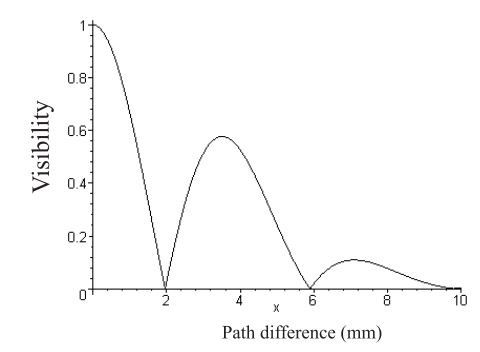
\includegraphics[scale=0.6]{EOQ14.JPG}
\end{figure}
\end{qns}
\begin{ans}
By the Wiener-Khinchine theorem, the power spectrum $P(\omega)$ is related to the Fourier transform of the visibility $\mathcal{F}[V(\tau)]$ where $\tau$ is related to the path difference $c\tau$. If the shell of the star is not expanding, the power spectrum will just be a Gaussian due to thermal broadening with linewidth $2.36\sigma$, where $\sigma=\frac{\omega_0}{c}\sqrt{\frac{k_BT}{m}}$. The expansion causes an overall shift in frequency due to the Doppler effect $\Delta\omega=\frac{\omega_0v}{c}$ where $v$ is the velocity of the expansion. This is manifested in the power spectrum by a shift in $\omega$-space, i.e. convolve the centred Gaussian with a pair of delta functions $\delta(\omega_0-\Delta\omega)+\delta(\omega_0+\Delta\omega)$. The power spectrum is then
$$P(\omega)\sim e^{-\omega^2/2\sigma}*\bigg[\delta(\omega_0-\Delta\omega)+\delta(\omega_0+\Delta\omega)\bigg]$$
giving a visibility profile of
$$V(\tau)\sim e^{-\sigma^2\tau^2/2}\cos(\Delta\omega~\tau)$$
The visibility is exactly zero when $\cos(\Delta\omega~\tau)=0$ at $\Delta\omega~\tau=\pi/2$. From the graph, we have $c\tau=2$ mm. Hence, from the Doppler shift, we have
$$\frac{\omega_0v}{c}=\Delta\omega=\frac{\pi}{2\tau}=\frac{\pi c}{2(2\times10^{-3})}\implies v=\frac{\pi}{2}\frac{c^2}{\omega_0(2\times10^{-3})}=\frac{\lambda_0c}{4}\frac{1}{2\times10^{-3}}=24.6~km/s$$
The coherent length $\ell_c$ is the path difference at which the visibility falls by $1/e=0.63$. From graph, we have $\ell-c=3.6$ mm. The frequency linewidth is 
$$\delta\omega=2.36\sigma\approx\frac{2.36\sqrt{2}c}{\ell_c}=\frac{2.36\sqrt{2}}{3.6\times10^{-3}}c=2.78\times10^{11}s^{-1}$$
If the linewidth is solely due to thermal broadening, we have
$$\sigma=\omega_0\sqrt{\frac{k_BT}{mc^2}}=\frac{c\sqrt{2}}{\ell_c}\implies T=\frac{\lambda_0^22c^2m}{(2\pi)^2\ell_c^2k_B}=\frac{(656\times10^{-9})^22(3\times10^8)^2(1.67\times10^{-27})}{(2\pi)^2(3.6\times10^{-3})^2(1.38\times10^{-23}}=18300 K$$
\textcolor{red}{value too large?}
\end{ans}
\newpage
\begin{qns}[Temporal coherence]
A Michelson interferometer forms fringes with cadmium red light of wavelength 643.847 nm and linewidth 0.0013 nm.
\begin{enumerate}[label=(\alph*)]
\item Estimate the coherence length for the light.
\item  Estimate the visibility of the fringes when one mirror is moved by distances $d= 10 mm$ and 50 mm from the position of zero path difference between the arms.
\item If the line-shape were a top-hat function, at what mirror position $d$ would the visibility first fall to zero?
\end{enumerate}
\end{qns}
\begin{ans}\leavevmode
\begin{enumerate}[label=(\alph*)]
\item The frequency linewidth is $\delta\omega=2.36\sigma$, but
$$\delta\omega=2\pi c\delta(1/\lambda)\sim2\pi c\delta\lambda/\lambda^2$$
The coherence length is
$$\ell_c\sim\frac{c\sqrt{2}}{\sigma}\sim c\sqrt{2}\frac{2.36}{2\pi c}\frac{\lambda^2}{\delta\lambda}=\frac{2.36}{\pi\sqrt{2}}\frac{643.847^2}{0.0013}10^{-9}=0.169m$$
\item the visibility is
$$V=\exp(-2\sigma^2d^2/c^2)\approx\exp(-(2d)^2/\ell_c^2)$$
The path difference $2d$ will then be 20 mm and 100 mm:
$$V(d=10)\approx\exp(-0.02^2/0.16^2)=0.98,\quad V(d=50)\approx\exp(-0.1^2/0.16^2)=0.68$$
\item The line-shape is a top-hat function centred at $\omega_0$ and width $\delta\omega=2\pi c\delta\lambda/\lambda^2$. Its Fourier transform will be a sinc curve $\sinc(\delta\omega t/2)$. The first zero occurs at $(t\delta\omega/2)=\pi$. We have $2d=ct$ and so
$$d=\frac{\pi c}{\delta\omega}=\frac{\lambda^2}{2\delta\lambda}=\frac{643.847^2}{0.0013}10^{-9}=0.16 m$$
\end{enumerate}
\end{ans}
\begin{qns}[Spatial coherence]
A long hot wire of width $w = 0.1$ mm is placed in the focal plane of a lens of focal length $f = 100$ mm. Light from the glowing wire passes through the lens and a filter which transmits only a very small range of wavelengths near $\lambda=600$ nm, and falls onto a screen placed normal to the axis behind the lens. Show that the degree of lateral coherence $\gamma$ for light arriving at two points on the screen separated by $d$ in a direction perpendicular to the wire is:
$$\gamma(d)=\sinc\frac{\pi wd}{f\lambda}$$
What is the smallest separation $d$ for which the degree of coherence is zero?
\end{qns}
\begin{ans}
The van Cittert-Zernike theorem states that the degree of lateral coherence is the Fourier transform of the angular intensity distribution of the source $I(\theta)$, i.e.
$$\gamma(u)=\frac{1}{I_0}\int I(\theta)e^{-iu\theta}d\theta$$
The intensity profile $I(\theta)$ is a top-hat function with maximum angular span $\theta=\pm\frac{w}{2f}$, so
$$\gamma(u)=\frac{1}{I_0}\int_{-w/2f}^{w/2f}I_0e^{-iu\theta}d\theta=-\frac{1}{i}\bigg[\frac{e^{-iuw/2f}}{w/2f}-\frac{e^{iuw/2f}}{-w/2f}\bigg]=\sinc\frac{uw}{2f}$$
But $u=kd$, so $\gamma(d)=\sinc\frac{\pi dw}{\lambda f}$. The first zero occurs at 
$$\frac{wd}{f\lambda}=1\implies d=\frac{f\lambda}{w}=\frac{(100\times10^{-3})(600\times10^{-9})}{0.1\times10^{-3}}=0.6mm$$
\end{ans}
\newpage
\section{Problem Sheet 2}
\subsection*{Electrodynamics}
\begin{qns}[Magnetic vector potential]
Starting from the relevant expressions for the magnetic field components
$$B_r=\frac{\mu_0m\cos\theta}{2\pi r^3},\quad B_\theta=\frac{\mu_0m\sin\theta}{4\pi r^3}$$
find a magnetic vector potential $\mathbf{A}(\mathbf{r})$ suitable for describing the fields due to a static magnetic dipole moment $\mathbf{m}$ aligned along Oz.
\end{qns}
\begin{ans}
In spherical polars, we have
$$B_r=\frac{1}{r^2\sin\theta}\bigg[\frac{\partial}{\partial\theta}(rA_\phi\sin\theta)-\frac{\partial}{\partial\phi}(rA_\theta)\bigg],\quad B_\theta=\frac{1}{r\sin\theta}\bigg[\frac{\partial}{\partial\phi}A_r-\frac{\partial}{\partial r}(rA_\phi\sin\theta)\bigg],\quad B_\phi=\frac{1}{r}\bigg[\frac{\partial}{\partial r}(rA_\theta)-\frac{\partial}{\partial\theta} A_r\bigg]$$
We then solve
$$B_r=\frac{\mu_0m\cos\theta}{2\pi r^3}=\frac{1}{r^2\sin\theta}\frac{\partial}{\partial\theta}(rA_\phi\sin\theta)\implies rA_\phi\sin\theta=-\frac{\mu_0m}{8\pi r}\cos2\theta+f(r,\phi)=-\frac{\mu_0m}{8\pi r}+\frac{\mu_0m}{4\pi r}\sin^2\theta+f(r,\phi)$$
$$B_\theta=\frac{\mu_0m\sin\theta}{4\pi r^3}=\frac{-1}{r\sin\theta}\frac{\partial}{\partial r}(rA_\phi\sin\theta)\implies rA_\phi\sin\theta=-\frac{\mu_0m\sin^2\theta}{4\pi r^2}+g(\theta,\phi)$$
Comparing gives $f(r,\phi)=\frac{\mu_0m}{8\pi r}$ and $g(\theta,\phi)=0$, hence
$$\mathbf{A}=\frac{\mu_0m\sin\theta}{4\pi r^2}\boldsymbol{\hat{\phi}}$$
\end{ans}
\begin{qns}[Magnetic vector potential]
Show that (b) below represents the components of a real magnetic field, whereas (a) does not. For the case (b) find the current density distribution $\mathbf{J}$ required to produce the field, and the corresponding vector potential $\mathbf{A}$.
\begin{enumerate}[label=(\alph*)]
\item $\frac{B_0b}{r^3}((x-y)z,(x-y)z,x^2-y^2)$ in Cartesian co-ordinates.
\item $B_0b^2(zr/(b^2+z^2)^2,0,1/(b^2+z^2))$ in cylindrical polar coordinates.
\end{enumerate}
\end{qns}
\begin{ans}
The general procedure is to first check $\mathbf{B}$ satisfies $\boldsymbol{\nabla}\cdot\mathbf{B}=0$. otherwise, the magnetic field is not physical.
\begin{enumerate}[label=(\alph*)]
\item We see that this given magnetic field is not physical: 
\begin{align}
    \boldsymbol{\nabla}\cdot\mathbf{B}&=B_0b\bigg[\frac{\partial}{\partial x}\bigg(\frac{(x-y)z}{r^3}\bigg)+\frac{\partial}{\partial y}\bigg(\frac{(x-y)z}{r^3}\bigg)+\frac{\partial}{\partial z}\bigg(\frac{x^2-y^2}{r^3}\bigg)\bigg]\nonumber\\
    &=B_0b\bigg[\frac{z}{r^3}-\frac{3x^2z}{r^5}+\frac{3xyz}{r^5}-\frac{z}{r^3}-\frac{3xzy}{r^5}+\frac{3y^2z}{r^5}+\frac{x-y}{r^3}-\frac{3z^2x}{r^5}+\frac{3z^2y}{r^5}\bigg]\nonumber\\
    &=B_0b\bigg[-\frac{3x^2z}{r^5}+\frac{3y^2z}{r^5}+\frac{x-y}{r^3}-\frac{3z^2x}{r^5}+\frac{3z^2y}{r^5}\bigg]\neq 0\nonumber
\end{align}
\item This field is physical!
$$\boldsymbol{\nabla}\cdot\mathbf{B}=B_0b^2\bigg[\frac{1}{r}\frac{\partial}{\partial r}\bigg(\frac{r^2z}{(b^2+z^2)^2}\bigg)+\frac{\partial}{\partial z}\bigg(\frac{1}{b^2+z^2}\bigg)\bigg]=B_0b^2\bigg[\frac{1}{r}\frac{2rz}{(b^2+z^2)^2}-\frac{2z}{(b^2+z^2)^2}\bigg]=0$$
Next, use Ampere's Law to find the current source $\mathbf{J}$:
$$\boldsymbol{\nabla}\times\mathbf{B}=\mu_0\mathbf{J},\quad B_r=\frac{rz}{(b^2+z^2)^2},\quad B_\phi=0,\quad B_z=\frac{1}{b^2+z^2}$$
$$\implies J_r=\frac{B_0b^2}{\mu_0}\bigg[\frac{1}{r}\frac{\partial B_z}{\partial\phi}-\frac{1}{r}\frac{\partial(rB_\phi)}{\partial z}\bigg]=\frac{B_0b^2}{\mu_0r}\frac{\partial}{\partial\phi}\frac{1}{b^2+z^2}=0,\quad J_z=\frac{1}{r}\frac{\partial}{\partial r}(rB_\phi)-\frac{1}{r}\frac{\partial B_r}{\partial\phi}=0$$
$$J_\phi=\frac{\partial B_r}{\partial z}-\frac{\partial B_z}{\partial r}=\frac{B_0b^2r}{\mu_0}\frac{(b^2+z^2)^2-2z(b^2+z^2)2z}{(b^2+z^2)^4}=\frac{r(b^2-3z^2)}{(b^2+z^2)^3}\frac{B_0b^2}{\mu_0}$$
By Poisson's equation, we have $\nabla^2\mathbf{A}\propto\mathbf{J}$, hence $\mathbf{J}$ only has non-zero component in the $\phi$ direction:
$$B_r=-\frac{1}{r}\frac{\partial}{\partial z}(rA_\phi)\implies rA_\phi=\frac{B_0b^2r^2}{2(b^2+z^2)}+f(r,\phi)$$
$$B_z=\frac{1}{r}\frac{\partial}{\partial r}(rA_\phi)\implies rA_\phi=\frac{B_0b^2r^2}{2(b^2+z^2)}+g(z,\phi)$$
Comparing gives $f=g=0$, and hence $\mathbf{A}=\frac{B_0b^2r}{2(b^2+z^2)}\boldsymbol{\hat{\phi}}$.
\end{enumerate}
\end{ans}
\subsection*{Radiation}
\begin{qns}[Dipole radiation]
A dipole antenna is enclosed in a sealed plastic box and radiates at a wavelength of 10 cm. Suggest (non-destructive) experiments to determine its orientation and whether it is an electric or a magnetic dipole.\\[5pt]
How could this information be deduced if the dipole antenna is disconnected from any power supply and its terminals shorted with a matched load?
\end{qns}
\begin{ans}
For $\lambda=10$ cm, the far field approximation is valid at least several metres away. We can use the dipole antenna as a radiation detector, by moving the source of known directionality. Whenever no radiation is detected, we are in line with the dipole. Now if we detect perpendicular to that direction (staying in the far field limit):
\begin{itemize}
    \item if the dipole is electric: $\mathbf{B}$ field is azimuthal, with $\mathbf{E}$ field in $\theta$ direction
    \item if the dipole is magnetic: $\mathbf{E}$ field is azimuthal, with $\mathbf{B}$ field in $\theta$ direction.
\end{itemize}
This can be differentiated by the motion of a charge (Lorentz force law), or by taking voltage measurements across a dielectric placed in the field.\\[5pt]
For the case where the dipole antenna is shorted with a matched load, the power delivered to the matched load resistor is half the incident power from the EM wave. We distinguish electric and magnetic dipole using the radiation resistance $R_r$: first compute for the electric dipole scenario, i.e.
$$\langle P^{\text{ED}}\rangle=\frac{\omega^4p_0^2}{12\pi\varepsilon_0c^3}=\frac{\omega^2\langle\dot{p}^2\rangle}{6\pi c^3\varepsilon_0}=\frac{\omega^2d^2\langle I^2\rangle}{6\pi c^2\varepsilon_0}$$
where $\dot{p}=-i\omega p_0e^{-i\omega_0t}$ such that $\langle\dot{p}^2\rangle=\frac{1}{2}\omega^2p_0^2$. The radiation resistance is
$$R_r^{\text{ED}}=\frac{\langle P^{\text{ED}}\rangle}{\langle I^2\rangle}=\frac{\omega^2d^2}{6\pi c\varepsilon_0}\bigg(\frac{2\pi}{\lambda}\bigg)^2=\frac{2\pi}{3}Z_0\frac{d^2}{\lambda^2}$$
For the magnetic dipole case
$$\langle P^{\text{MD}}\rangle=\frac{\mu_0\omega^4m_0^2}{12\pi c^3}=\frac{\mu_0\omega^2\langle\dot{m}^2\rangle}{6\pi c^3}=\frac{\mu_0d^4\omega^2\langle\dot{I}^2\rangle}{6\pi c^3}=\frac{\mu_0d^4\omega^4\langle I^2\rangle}{6\pi c^3}$$
and the corresponding radiation resistance is
$$R_r^{\text{MD}}=\frac{d^4}{6\pi c\varepsilon_0}\bigg(\frac{2\pi}{\lambda}\bigg)^2=(2\pi)^2\frac{2\pi}{3}Z_0\frac{d^4}{\lambda^4}$$
So we vary the wavelength of the incoming light, if the radiation resistance show a $1/\lambda^2$ dependence, then the dipole antenna is an electric dipole. Otherwise, if $R_r\propto\lambda^{-4}$, then the dipole antenna is a magnetic dipole. Finally, for the orientation, this can be found by shining plane-polarized light, since $\langle P_{\text{load}}\rangle\propto\sin^2\theta$. Whenever there is zero power delivered to the load, the incoming light ray is parallel to the dipole.
\end{ans}
\newpage
\begin{qns}[Magnetic dipole radiation]
A magnetic dipole at the origin lies in the x-y-plane and is rotating at constant angular frequency about the $z$-axis.
\begin{enumerate}[label=(\alph*)]
\item Show that in the x-y-plane the radiation pattern is circular and the emitted radiation is polarized parallel to Oz.
\item What is the polarization of the radiation emitted at an angle $\theta$ to the rotation axis Oz?
\end{enumerate}
\end{qns}
\begin{ans}\leavevmode
\begin{enumerate}[label=(\alph*)]
\item We have $\mathbf{n}$ to be the unit vector in spherical coordinates, pointing in the direction from the origin to the point of interest. Due to axial symmetry, we have $\phi=0$, and so
$$\mathbf{n}=\begin{pmatrix}\sin\theta\\0\\\cos\theta\\\end{pmatrix}$$
The magnetic dipole is
$$\mathbf{m}=\begin{pmatrix}m_0\cos\omega t\\m_0\sin\omega t\\0\\\end{pmatrix}$$
The magnetic vector potential that corresponds to magnetic dipole radiation is
$$\mathbf{A}=\frac{ik\mu_0}{4\pi}(\mathbf{n}\times\mathbf{m})\frac{e^{ikr}}{r}$$
The magnetic and electric fields are
$$\mathbf{B}=\boldsymbol{\nabla}\times\mathbf{A}=\frac{\mu_0k^2}{4\pi}[(\mathbf{n}\times\mathbf{m})\times\mathbf{n}]\frac{e^{ikr}}{r},\quad\mathbf{E}=\frac{iZ_0}{k\mu_0}\boldsymbol{\nabla}\times\mathbf{B}=-\frac{Z_0k^2}{4\pi}(\mathbf{n}\times\mathbf{m})\frac{e^{ikr}}{r}$$
We have
$$\mathbf{E}(r,t)\propto(\mathbf{n}\times\mathbf{m})=\begin{pmatrix}\mathbf{\hat{x}}&\mathbf{\hat{y}}&\mathbf{\hat{z}}\\\sin\theta&0&\cos\theta\\m_0\cos\omega t&m_0\sin\omega t&0\\\end{pmatrix}=\begin{pmatrix}-m_0\cos\theta\sin\omega t\\m_0\cos\theta\cos\omega t\\m_0\sin\theta\sin\omega t\\\end{pmatrix}$$
At special time points, we have
$$\mathbf{E}(r,\omega t=0)\propto\begin{pmatrix}0\\m_0\cos\theta\\0\\\end{pmatrix},\quad\mathbf{E}(r,\omega t=\pi/2)\propto\begin{pmatrix}-m_0\cos\theta\\0\\m_0\sin\theta\\\end{pmatrix}$$
When $\theta=\pi/2$, the radiation is linearly polarized with polarization axis along the $z$-axis. We have $\mathbf{E}(r,t)\propto(0,0,m_0\sin\omega t)$, i.e. the radiation field at a given radius is of constant amplitude.
\item At $\theta\neq 0,\pi/2$, the radiation is elliptically polarized. Particularly, when $\theta=0$, the radiation is circularly polarized.
\end{enumerate}
\end{ans}
\newpage
\begin{qns}[Magnetic dipole]
A pulsar is can be represented as a constant magnetic moment $\mathbf{M}$ rotating with
an angular velocity $\omega$ in vacuum about an axis perpendicular to $\mathbf{M}$. By considering the rotating magnet as equivalent to two orthogonal magnets varying in phase quadrature, show that the energy loss due to radiation causes $\omega$ to obey the equation $\omega\ddot{\omega}=3\dot{\omega}^2$.\\[5pt]
[Assume the formula for radiation loss for a magnetic dipole, and that $\dot{\omega}<<\omega^2$.]\\[5pt]
For the pulsar in the Crab Nebula, the period $T = $33 ms and $\dot{T}=$ 36 ns/day. Assuming that it is a sphere (of uniform density) with radius 7 km and a mass equal to that of the Sun ($2\times 10^{30}$ kg), estimate $\mathbf{M}$ and hence the magnetic field at its equator.
\end{qns}
\begin{ans}
Model the rotating magnet as two orthogonal magnets varying in quadrature. The magnetization is $\mathbf{M}=M_1\mathbf{\hat{x}}+M_2\mathbf{\hat{y}}=M\cos\omega t\mathbf{\hat{x}}+M\sin\omega t\mathbf{\hat{y}}$. The time-averaged Poynting vector is
$$\langle\mathbf{N}\rangle=\langle(\mathbf{E_1}+\mathbf{E_2})\times(\mathbf{H_1}+\mathbf{H_2})\rangle=\langle\mathbf{E_1}\times\mathbf{H_1}\rangle+\langle\mathbf{E_2}\times\mathbf{H_2}\rangle=2\langle P_{\text{MD}}\rangle$$
where the time-averaged cross-terms vanish since $M_1$ and $M_2$ are in quadrature. By Poynting theorem, the average power loss is two times that of the single magnetic dipole. Since $\dot{\omega}<<\omega^2$, the energy loss in one period is small compared to the stored energy $E=\frac{1}{2}I\omega^2$.
$$\frac{1}{2}2I\omega\dot{\omega}=\frac{dE}{dt}=-\frac{\mu_0M^2\omega^4}{6\pi c^3}\implies I\ddot{\omega}=-\frac{3\mu_0M^2\omega^2}{6\pi c^3}\dot{\omega},\quad I\dot{\omega}=-\frac{\mu_0M^2}{6\pi c^3}\omega^3$$
Take the ratio of the above results, we have
$$\frac{\dot{\omega}}{\ddot{\omega}}=\frac{\omega}{3\dot{\omega}}\implies3\dot{\omega}^2=\ddot{\omega}\omega$$
We are given $T=33$ ms and $\dot{T}=36$ ns/day. We then have
$$\dot{\omega}=\frac{d}{dt}\frac{2\pi}{T}=-\frac{2\pi}{T^2}\dot{T}=-\frac{\omega^2}{2\pi}\dot{T}=-\frac{(2\pi/33\times10^{-3})^2}{2\pi}\frac{36\times10^{-9}}{24(3600)}=-2.404\times10^{-9}~rad/s$$
Comparing with $\omega^2=3.625\times10^4$ rad$^2$ s$^{-2}$, we have $\omega^2>>\dot{\omega}$ indeed. We then have
$$\dot{\omega}=-\frac{\mu_0M^2\omega^3}{6\pi c^3(2/5)mr^2}=-\frac{5\mu_0M^2\omega^3}{12\pi c^3mr^2}$$
$$\implies M=\sqrt{\frac{-12\pi c^3mr^2\dot{\omega}}{5\mu_0\omega^3}}=\sqrt{\frac{-12\pi (3\times10^8)^3(2\times10^{30})(7\times10^3)^2(-2.404\times10^{-9})}{5(4\pi\times10^{-7})(2\pi/33\times10^{-3})^3}}=2.35\times10^{27}Am^2$$
At $R=7$ km, we are indeed the far-field limit since
$$\frac{2\pi c}{\omega}=\frac{2\pi(3\times10^8)}{(2\pi/33\times10^{-3})}=9.9\times10^6>>R=7\times10^3$$
The equatorial radiation field of the magnetic dipole is then
$$B_\theta=\frac{\mu_0M}{4\pi R^3}\sin\theta=\frac{(4\pi\times10^{-7})(2.35\times10^{27})}{4\pi(7\times10^3)^3}\sin\theta=6.85\times10^8~\sin\theta$$
\end{ans}
\newpage
\begin{qns}[Antenna]
What are meant by the radiation resistance and power gain of an antenna? For an antenna which consists of a plane loop of wire of area $a^2$ operating at a frequency $\omega<<c/a$, calculate the radiation resistance and power gain.\\[5pt]
Radiation, linearly-polarized with its magnetic field perpendicular to the plane of the loop, is incident from a direction in that plane. Find the cross-section for combined scattering and absorption when the antenna is connected to a matched load.\\[5pt]
[Assume without proof that such a loop radiates mean power $\mu_0I_0^2\omega^4a^4/(12\pi c^3)$ when a current $I_0\cos\omega t$ flows in it.]
\end{qns}
\begin{ans}
When the antenna is connected to a driving circuit, it dissipates energy in the form of radiation. This dissipation can be modelled as a resistor with an effective resistance $R_r$. 
$$R_r=\frac{\langle P\rangle}{\langle I^2\rangle}$$
where $P$ is the total radiated power. Power gain describes the directionality of the emitted radiation
$$G(\theta,\phi)=\frac{N(\theta,\phi)}{(1/4\pi)\int N(\theta,\phi)d\Omega}$$
where $N(\theta,\phi)$ is the time-averaged radial Poynting flux. Given that the loop radiates mean power $\frac{\mu_0I_0^2\omega^4a^4}{12\pi c^3}$, the radiation resistance is
$$R_r=\frac{\langle P\rangle}{\langle I^2\rangle}=\frac{\mu_0I_0^2\omega^4a^4}{12\pi c^3}\frac{2}{I_0^2}=\frac{\mu_0\omega^4a^4}{6\pi c^3}$$
For a magnetic dipole, $N(\theta,\phi)\propto\sin^2\theta$, and so the power gain is
$$G(\theta,\phi)=\frac{A\sin^2\theta}{(A/4\pi)2\pi\int_0^\pi\sin^2\theta\sin\theta d\theta}=\frac{\sin^2\theta}{(1/2)(4/3)}=\frac{3}{2}\sin^2\theta$$
By Faraday's law, the potential difference induced by the oscillating $B$ field is $a^2\dot{B}$, so
$$\langle V^2\rangle=a^4\omega^2\langle B^2\rangle$$
The time-averaged incident Poynting flux is
$$\langle N_{\text{inc}}\rangle=\langle EH\rangle=\frac{c}{\mu_0}\langle B^2\rangle$$
The total mean power for a matched load is
$$\langle P_{\text{tot}}\rangle=\frac{\langle V^2\rangle}{2R_r}=\frac{a^4\omega^2\langle B^2\rangle6\pi c^3}{2\mu_0\omega^4a^4}=\frac{3\pi c^3\langle B^2\rangle}{\omega^2\mu_0}=\frac{3\pi c^2}{\omega^2}\langle N_{\text{inc}}\rangle$$
The effective area (or the cross-section) is
$$A_{\text{eff}}=\frac{\langle P_{\text{tot}}\rangle}{\langle N_{\text{inc}}\rangle}=\frac{3\pi c^2}{\omega^2}$$
\end{ans}
\newpage
\begin{qns}[Scattering]
Estimate the number of molecules above each m$^2$ of the Earth’s surface. Hence, on the assumption that a molecule can be represented as a perfectly conducting sphere of radius 0.1 nm, estimate the reduction in the (ultra-violet) radiation with wavelength $\lambda=$ 320 nm arriving from the Sun at noon on the Equator due to scattering by the atmosphere.

[Assume that half of the radiation scattered still reaches the Earth’s surface and ignore multiple scattering.]
\end{qns}
\begin{ans}
The number density profile is an exponential fall off, i.e.
$$n=n_0e^{-mgh/k_BT},\quad n_0=\frac{N_A}{22.4\times10^{-3}m^{3}}\text{ at STP}$$
The total number per unit area is
$$N=n_0\int_0^\infty e^{-mgh/k_BT}dh=\frac{n_0k_BT}{mg}[e^{-mgh/k_BT}]_0^\infty=\frac{N_Ak_BT}{mg}\frac{1}{22.4\times10^{-3}m^3}=2.44\times10^{29}m^{-2}$$
Using ideal gas law, we have
$$\frac{N}{A}=\frac{0.5p_0h}{k_BT}=\frac{10^5(16000)}{2(1.38\times10^{-23})(288)}=2.01\times10^{29}\text{ atoms }m^{-2}$$
where half of the radiation scattered reaches Earth. Since $\lambda=320 nm>>0.1 nm$ (radius of the scatterers), the type of scattering is Rayleigh scattering with cross-section $\sigma=\frac{8\pi^3\mu_0^2c^4\alpha^2}{3\lambda^4}$. The ratio of power lost to incoming power is
\begin{align}
    \frac{\langle P_{\text{lost}}\rangle}{\langle P_{\text{incoming}}\rangle}&=\frac{\langle P_{\text{scattered}}\rangle}{2\langle P_{\text{incoming}}\rangle}\nonumber\\&=\frac{\sigma N}{2A}\nonumber\\&=\frac{8\pi^3\mu_0^2c^4(4\pi r^3\varepsilon_0)^2}{3\lambda^4}\frac{N}{2A}\nonumber\\&=\frac{128\pi^5r^6}{3\lambda^4}\frac{N}{2A}\nonumber\\&=\frac{128\pi^5}{3}\frac{(0.1\times10^{-9})^6}{(320\times10^{-9})^4}\frac{1}{2}(2.44\times10^{29})\nonumber\\&=0.15\nonumber
\end{align}
where $\alpha=4\pi r^3\varepsilon_0$ for a perfectly conducting sphere.
\end{ans}
\begin{qns}[Scattering]
Estimate the degree of polarization of the overhead sky at noon on a clear spring day (say March 21) in Cambridge.
\end{qns}
\begin{ans}
At Cambridge, the latitude is $\phi=+53\degree$. At Equinox (Mar 21), we may ignore Earth's axial tilt. We are also given that the Sun is overhead and so sunlight arriving parallel to the equator, is scattered by the atmosphere through an angle $52$ degrees. The degree of polarization is
$$\frac{I_{\text{max}}-I_{\text{min}}}{I_{\text{max}}+I_{\text{min}}}=\frac{1-\cos^2\phi}{1+\cos^2\phi}=0.454$$
where $\phi$ is the latitude of the observer. 
\end{ans}
\newpage
\section{Problem Sheet 3}
\subsection*{Relativistic Electrodynamics}
\begin{qns}[4-vector]\leavevmode
\begin{enumerate}[label=(\roman*)]
\item Prove that the inner product $\mathbf{A}\cdot\mathbf{B}$ of two 4-vectors $\mathbf{A}$ and $\mathbf{B}$ is Lorentz invariant.
\item Prove that if $\mathbf{A}\cdot\mathbf{B}$ is Lorentz invariant and $\mathbf{A}$ is a 4-vector, then $\mathbf{B}$ is also a 4-vector.
\end{enumerate}
\end{qns}
\begin{ans}
For this question, we explicitly demonstrate this using the convention for the Minkowski metric $\eta=\diag(+1,-1,-1,-1)$. The results will still hold even with the other convention choice.
\begin{enumerate}[label=(\roman*)]
\item The inner product of two four-vectors is explicitly given as
$$A\cdot B=A_0B_0-A_1B_1-A_2B_2-A_3B_3$$
The transformation of these four-vectors follow the Lorentz transformation:
$$\Lambda=\begin{pmatrix}\gamma&-\gamma\beta&0&0\\-\gamma\beta&\gamma&0&0\\0&0&1&0\\0&0&0&1\\\end{pmatrix},\quad A'=\Lambda A=\begin{pmatrix}\gamma A_0-\gamma\beta A_1\\-\gamma\beta A_0+\gamma A_1\\A_2\\A_3\\\end{pmatrix},\quad B'=\Lambda B=\begin{pmatrix}\gamma B_0-\gamma\beta B_1\\-\gamma\beta B_0+\gamma B_1\\B_2\\B_3\\\end{pmatrix}$$
so the inner product transforms like
\begin{align}
A'\cdot B'&=(\gamma A_0-\gamma\beta A_1)(\gamma B_0-\gamma\beta B_1)-(-\gamma\beta A_0+\gamma A_1)(-\gamma\beta B_0+\gamma B_1)-A_2B_2-A_3B_3\nonumber\\&=A_0B_0\gamma^2(1-\beta^2)-A_1B_1\gamma^2(-\beta^2+1)-A_2B_2-A_3B_3\nonumber\\&=A\cdot B\nonumber
\end{align}
Hence, the inner product is invariant under Lorentz transformation.
\item Similarly, suppose $A\cdot B=A'\cdot B$, but we are only given that $A$ is a 4-vector and thus its transformation is given by the Lorentz transformation. We have
$$A\cdot B=A_0B_0-A_1B_1-A_2B_2-A_3B_3$$
$$A'\cdot B'=(\gamma A_0-\gamma\beta A_1)B_0'-(\gamma A_1-\gamma\beta A_0)B_1'-A_2B_2'-A_3B_3'$$
Comparing coefficients give:
$$B_3=B_3',\quad B_2=B_2',\quad -B_1=-\gamma\beta B_0'-\gamma B_1',\quad B_0=\gamma B_0'+\gamma\beta B_1'\implies B'=\Lambda B$$
\end{enumerate}
\end{ans}
\newpage
\begin{qns}[Maxwell's equations, relativistic kinematics]
In the standard arrangement of co-ordinate frames, a slab of non-dispersive medium with refractive index $n$ is at rest in $S'$ and has thickness $d$ in the Oz' direction. In the laboratory frame $S$ the slab moves along the x-axis with speed $v = \beta c$.
\begin{enumerate}[label=(\roman*)]
\item Show that, for light moving through the slab parallel to its motion, the refractive index as determined in $S$ is:
$$n_v=\frac{n+\beta}{n\beta+1}\approx n-(n^2-1)\beta \text{ for small }\beta$$
\item Show that a ray of light falling on the slab at normal incidence in $S$ passes through the slab at an angle $\alpha=\sin^{-1}(\beta/n)$ to the Oz' axis as measured in $S'$. Hence show that in frame $S$ the ray is laterally displaced by a distance:
$$a=\gamma d~\beta\frac{n^2-1}{\sqrt{n^2-\beta^2}}$$
after passing through the slab. [$\gamma=1/\sqrt{1-\beta^2}$]
\end{enumerate}
\end{qns}
\begin{ans}\leavevmode
\begin{enumerate}[label=(\roman*)]
\item The refractive index of a medium can be obtained from the speed of the electromagnetic wave travelling in this medium. For simplicity, assume the medium is isotropic with refractive index $n$ in $S'$. The electromagnetic wave is a solution to the Maxwell's equations in this medium. For a sinusoidal solution (EM wave), we plug this to any one of the Maxwell's equation, say
$$\boldsymbol{\nabla}\times\mathbf{E}=-\mathbf{\dot{B}}\implies ik\mathbf{E}=i\omega\mathbf{B}\implies E_x=\frac{\omega}{k}B_y=\frac{c}{n}B_y$$
In frame $S'$, we thus have $E_x'/B_y'=c/n$. But the Maxwell's equations are covariant and must be true in all inertial frames. Hence, $E_x/B_y=c/n_v$ in frame $S$ for some $n_v$. The transverse electromagnetic fields (perpendicular to the boost in the $z$ direction) transform like
$$E_x'=\gamma(E_x-vB_y),\quad B_y'=\gamma\bigg(B_y-\frac{v}{c^2}E_x\bigg)$$
with
$$\frac{c}{n}=\frac{E_x'}{B_y'}=\frac{E_x-vB_y}{B_y-(v/c^2)E_x}\implies\frac{E_x}{B_y}=\frac{c(1+n\beta)}{n+\beta}\implies n_v=\frac{n+\beta}{1+n\beta}\approx(n+\beta)(1-n\beta)=n-(n^2-1)\beta$$
\item The ray is normal to the slab in frame $S$ but is inclined at an angle $\theta_i$ in frame $S'$. Since the slab is moving, we must have
$$\sin\theta_i=\frac{v}{c}=\beta$$
but staying in the rest frame of the slab, we apply Snell's Law
$$n\sin\alpha=\sin\theta_i\implies\alpha=\sin^{-1}(\beta/n)$$
The dimension of the slab perpendicular to the boost, i.e. its thickness, is unchanged. Since the angle of refraction is $\alpha$, then by geometry, the lateral displacement of the ray in the medium is
$$\Delta x'=-d\tan\alpha=-\frac{\beta d}{\sqrt{n^2-\beta^2}}$$
The time taken in frame $S'$ for the ray to travel from the top to the bottom is
$$\Delta t'=\frac{\sqrt{d^2+(\Delta x')^2}}{c/n}=\sqrt{d^2+\frac{d^2\beta^2}{n^2-\beta^2}}\frac{n}{c}=\frac{dn^2}{c}\frac{1}{\sqrt{n^2-\beta^2}}$$
Perform inverse Lorentz transformation to find this lateral displacement in frame $S$:
$$\Delta x=\gamma(\Delta x'+\beta c\Delta t')=\gamma\bigg[\frac{-\beta d}{\sqrt{n^2-\beta^2}}+\frac{\beta n^2d}{\sqrt{n^2-\beta^2}}\bigg]=\frac{\gamma\beta d}{\sqrt{n^2-\beta^2}}(n^2-1)$$
\end{enumerate}
\end{ans}
\newpage
\begin{qns}[Maxwell's equations, relativistic kinematics]
A particle with charge $q$ and rest mass $m$ moves in an electric field $\mathbf{E}$ and magnetic field $\mathbf{B}$. Show that its 4-velocity is $(\gamma c,\mathbf{\tilde{u}}c)$, where $\frac{d\mathbf{r}}{d\tau}=c\tilde{\mathbf{u}}$ and $\tau$ is the proper time measured by an observer moving with the particle. [Note that $\tilde{\mathbf{u}}$ is not the 3-velocity $\mathbf{u}$.]\\[5pt]
Show also that the particle’s equation of motion can be written in the form
\begin{align}
    \frac{d\tilde{u}}{d\tau}&=\frac{q}{mc}(\gamma\mathbf{E}+c\tilde{\mathbf{u}}\times\mathbf{B})\nonumber\\
    \frac{d\gamma}{d\tau}&=\frac{q}{mc}\mathbf{E}\cdot\mathbf{\tilde{u}}\nonumber
\end{align}
\end{qns}
\begin{ans}
The 4-position is defined as $X=(ct,\mathbf{x})$, where $\mathbf{x}$ is the 3-position. The 4-velocity is then defined to be $U=dX/d\tau$, where $\tau$ is the proper time.
$$U=\begin{pmatrix}c\frac{dt}{d\tau}\\\frac{d\mathbf{x}}{d\tau}\\\end{pmatrix}=\begin{pmatrix}\gamma c\\\mathbf{\tilde{u}}c\\\end{pmatrix}$$
where $dt/\gamma=d\tau$ follows from the definition of proper time. After extremizing some action (which we will omit the proof), one obtain the equation of motion in terms of the electromagnetic field strength tensor:
\begin{align}
m\frac{dU}{d\tau}&=qF^{\alpha\beta}U_\beta\nonumber\\
\implies m\begin{pmatrix}c\frac{d\gamma}{d\tau}\\c\frac{d\mathbf{\tilde{u}}}{d\tau}\\\end{pmatrix}&=q\begin{pmatrix}\mathbf{E}\cdot\mathbf{\tilde{u}}\\\gamma\mathbf{E}+c\mathbf{\tilde{u}}\times\mathbf{B}\\\end{pmatrix}\nonumber
\end{align}
\end{ans}
\begin{qns}[Relativistic electrodynamics]\leavevmode
\begin{enumerate}[label=(\roman*)]
\item A parallel plate capacitor is at rest in $S'$ with its plates perpendicular to Oy'. One
plate at $y'=0$ has zero potential and the other at $y'=s$ is at potential $−V_0$. Write down the 4-potential between the plates in $S'$. Transform the 4-potential to the frame $S$ in which the capacitor is moving at speed $c\beta$ along the positive $x$-direction. Hence find $\mathbf{E}$ and $\mathbf{B}$ between the plates in $S$, and interpret your results.
\item Repeat (i) when the plates are perpendicular to Ox' with the plate at $x'=0$ at zero potential and the other at $x'=s$ at potential $-V_0$.
\end{enumerate}
Are the results for (i) and (ii) consistent when two such perpendicularly oriented capacitors are considered together in $S'$, electrically connected in parallel?
\end{qns}
\begin{ans}\leavevmode
\begin{enumerate}[label=(\roman*)]
\item In frame $S'$, the capacitor is at rest. With a uniform electric field in the $y'$ direction, the potential linearly depends on $y'$, i.e. $\phi'=-V_0y'/s$, where $\phi(y'=0)=0$ and $\phi'(y'=s)=-V_0$. Note we are only interested in the region between the plates, i.e. $0\leq y'\leq s$. The 4-potential will then be
$$\mathcal{A}'=\begin{pmatrix}\phi/c\\\mathbf{A'}\\\end{pmatrix}=\begin{pmatrix}-\frac{V_0y'}{cs}\\\boldsymbol{0}\\\end{pmatrix}$$
where the 3-vector potential $\mathbf{A}$ is zero since there is no currents. To find the 4-potential in frame $S$, we perform an inverse Lorentz transformation:
$$\mathcal{A}=\Lambda^{-1}\mathcal{A}'=\begin{pmatrix}\gamma&\beta\gamma&0&0\\\beta\gamma&\gamma&0&0\\0&0&1&0\\0&0&0&1\\\end{pmatrix}\begin{pmatrix}-V_0y'/cs\\0\\0\\0\\\end{pmatrix}=\begin{pmatrix}-\gamma V_0y'/cs\\-\beta\gamma V_0y'/cs\\0\\0\\\end{pmatrix},\quad 0\leq y'\leq s$$
The potentials are then $\phi=-\frac{\gamma V_0y}{s},~\mathbf{A}=-\frac{\beta\gamma V_0y}{cs}\mathbf{\hat{x}}$. It follows that the electromagnetic fields are
$$\mathbf{E}=-\mathbf{\dot{A}}-\boldsymbol{\nabla}\phi=\frac{\gamma V_0}{s}\mathbf{\hat{y}},\quad\mathbf{B}=\boldsymbol{\nabla}\times\mathbf{A}=\frac{\beta\gamma V_0}{cs}\mathbf{\hat{z}}\neq\boldsymbol{0}$$
The electric field is unchanged since $y'=y$, i.e. perpendicular to the boost. In frame $S$, the magnetic field is non-zero, indicating that there is a current induced (in the $z$ direction) due to its relativistic motion, between the plates.
\item By a similar classical electrostatics argument, the 4-potential in frame $S'$ (where the capacitor is at rest) is
$$\mathcal{A}'=\begin{pmatrix}\frac{-V_0x'}{cs}\\\boldsymbol{0}\\\end{pmatrix}$$
where again the 3-vector potential $\mathbf{A}$ is zero since there is no currents. To find the 4-potential in frame $S$, again perform an inverse Lorentz transformation.
$$\mathcal{A}=\Lambda^{-1}\mathcal{A}'=\begin{pmatrix}\gamma&\beta\gamma&0&0\\\beta\gamma&\gamma&0&0\\0&0&1&0\\0&0&0&1\\\end{pmatrix}\begin{pmatrix}-V_0x'/cs\\0\\0\\0\\\end{pmatrix}=\begin{pmatrix}-\gamma V_0x'/cs\\-\beta\gamma V_0x'/cs\\0\\0\\\end{pmatrix},\quad 0\leq x'\leq s$$
but boosting the 4-position gives $x'=\gamma(x-\beta ct)$. It follows that the potentials are
$$\phi=-\frac{\gamma^2V_0}{s}(x-\beta ct),\quad\mathbf{A}=-\frac{\beta\gamma^2V_0}{cs}(x-\beta c)$$
The electromagnetic fields are then
$$\mathbf{E}=-\mathbf{\dot{A}}-\boldsymbol{\nabla}\phi=\bigg(-\frac{\beta\gamma^2V_0\beta c}{cs}+\frac{\gamma^2V_0}{s}\bigg)\mathbf{\hat{x}}=\frac{V_0}{s}\mathbf{\hat{x}}=\mathbf{E'},\quad\mathbf{B}=\boldsymbol{\nabla}\times\mathbf{A}=\boldsymbol{0}=\mathbf{B'}$$
This is expected since the Lorentz boost is now parallel to the electric field. The longitudinal electric field is not transformed and there is no induced magnetic field or current.
\end{enumerate}
In (ii), there is no current flow for both capacitors. In (i), the current flow is in a direction parallel to the plates and not through the loop. Hence, for both setups, there is no current and the situation is consistent.
\end{ans}
\begin{qns}[Relativistic electrodynamics]
Electric and magnetic fields, $\mathbf{E}$ and $\mathbf{B}$, as viewed in frame $S$ are such that when they are examined in frame $S'$, which is moving relative to $S$ with constant velocity $v$ along the common $x$-axis, the electric field is unaltered but the magnetic field is reversed. Show that the two fields are perpendicular in both frames and that, if $\mathbf{E} = (E_x, E_y, E_z)$, then
$$\mathbf{B}=\frac{\gamma-1}{\gamma v}(0,-E_z,E_y)$$
\end{qns}
\begin{ans}
We are given in frame $S'$ that
$$\mathbf{E'}=\mathbf{E},\quad\mathbf{B'}=-\mathbf{B}$$
The Lorentz boost is along the $x$ direction, so the electromagnetic fields (only the transverse ones non-trivially transform) transform like
$$E_\parallel'=E_\parallel,\quad \mathbf{E_\perp'}=\gamma(\mathbf{E}+(\mathbf{v}\times\mathbf{B}))_\perp\implies E_x'=E_x,~E_y'=\gamma(E_y-vB_z),~E_z'=\gamma(E_z+vB_y)$$
$$B_\parallel'=B_\parallel,\quad \mathbf{B_\perp'}=\gamma\bigg(\mathbf{B}-\frac{1}{c^2}(\mathbf{v}\times\mathbf{E})\bigg)_\perp\implies B_x'=B_x,~B_y'=\gamma\bigg(B_y+\frac{v}{c^2}E_z\bigg),~B_z'=\gamma(B_z-\frac{v}{c^2}E_y\bigg)$$
To ensure it satisfies the given transformed fields, we have
$$B_x=0,\quad B_z=\frac{\gamma-1}{\gamma v}E_y,\quad B_y=\frac{1-\gamma}{\gamma v}E_z,\quad E_x=E_x'$$
The magnetic field is then $\mathbf{B}=\frac{\gamma-1}{\gamma v}(0,-E_z,E_y)$. Take the dot product:
$$\mathbf{E}\cdot\mathbf{B}=(-E_yE_z+E_yE_z)\frac{\gamma-1}{\gamma v}=0,\quad\mathbf{E'}\cdot\mathbf{B'}=-\mathbf{E}\cdot\mathbf{B}=0$$
i.e. the fields are perpendicular in both frames.
\end{ans}
\newpage
\begin{qns}[Relativistic electrodynamics]
A plane conducting non-magnetic sheet of uniform thickness is oriented normal to the $y$ and $y'$ axes in frames $S$ and $S'$. $S'$ moves at a constant velocity $v$ in the positive $x$-direction in $S$, and the sheet is at rest in $S'$. In $S$, there is a uniform magnetic field having components $(0, 0, B)$, and the electric field is zero. Transform these fields to $S'$ and hence deduce:
\begin{enumerate}[label=(\alph*)]
\item the fields $\mathbf{E'_0}$ and $\mathbf{B'_0}$ outside the sheet;
\item the fields $\mathbf{E'_0}$ and $\mathbf{B'_0}$ inside the sheet;
\item the surface charge density in $S'$ on either side of the sheet.
\end{enumerate}
Transform the results for (b) back to $S$, and hence find $\mathbf{E}$ and $\mathbf{B}$ inside the sheet. Interpret these results from the point of view of an observer at rest in $S$.
\end{qns}
\begin{ans}\leavevmode
\begin{enumerate}[label=(\alph*)]
\item 

\item 

\item
\end{enumerate}
\end{ans}
\newpage
\subsection*{Radiation}
\begin{qns}
Derive expressions for the fields due to a uniformly moving charge.\\[5pt]
Two particles, each with charge $q$, are constrained to move with the same constant velocity $v$ parallel to the $x$-axis. Find the force on each due to the presence of the other when, instantaneously, one is at the origin and the other is at:
\begin{enumerate}[label=(\alph*)]
\item $(r, 0, 0)$;
\item $(0, r, 0)$;
\item $(r/\sqrt{2},r/\sqrt{2},0)$.
\end{enumerate}
\end{qns}
\begin{ans}\leavevmode
\begin{enumerate}[label=(\alph*)]
\item 

\item 

\item
\end{enumerate}
\end{ans}
\newpage
\begin{qns}\leavevmode
\begin{enumerate}[label=(\roman*)]
\item  By direct substitution, show that the quantities $|\mathbf{E}|^2-c^2|\mathbf{B}|^2$ and $\mathbf{E}\cdot\mathbf{B}$ are invariant under the Lorentz Transformations.
\item A region of space contains isotropic electromagnetic radiation of mean energy density $\langle U\rangle$. Show that an observer moving in the $x$-direction with speed $v$ through the region will measure a mean energy density $\langle U'\rangle$ and mean Poynting vector $\langle \mathbf{N'}\rangle$ given by
\end{enumerate}
\end{qns}
\begin{ans}\leavevmode
\begin{enumerate}[label=(\roman*)]
\item 

\item 

\end{enumerate}
\end{ans}
\begin{qns}
A 1 GeV electron passes into a region in which there is a transverse magnetic field of 1 T. Estimate the typical frequency of the synchrotron radiation emitted, and the fractional loss of energy per orbit.
\end{qns}
\begin{ans}

\end{ans}
\newpage
\begin{qns}
A particle of charge $q$ and rest mass $m$ is placed in an electromagnetic plane wave described by
$$E_y=cB_0\sin[\omega(t-x/c)],\quad E_x=E_z=0$$
$$B_z=B_0\sin[\omega(t-x/c)],\quad B_x=B_y=0$$
If the wave is `strong' (i.e. $qB_0/m\omega > 1$) it attains relativistic speeds and the force on it arising from the wave’s magnetic field cannot be ignored. Applying the results of Q.27, write down the equations of motion.\\[5pt]
If the particle is introduced at rest at $x = t = \tau = 0$, show that
\begin{enumerate}[label=(\alph*)]
\item $\tilde{u}_x=0$;
\item $\tilde{u}_x=\gamma-1$;
\item$(t-x/c)=\tau$, where $x$ refers to the particle's position at time $\tau$.
\end{enumerate}
Find the maximum energy $E_{\text{max}}$ attained by the particle and sketch its motion.
\end{qns}
\begin{ans}\leavevmode
\begin{enumerate}[label=(\alph*)]
\item 
\item 
\item
\end{enumerate}
\end{ans}
\end{document}